\documentclass{article}
\usepackage[frenchb]{babel}
\usepackage[utf8]{inputenc}
\usepackage[T1]{fontenc}
\usepackage{graphicx}
\usepackage{fancyhdr}

\pagestyle{fancy}
\title{Projet programmation par contrainte : Elisabeth}
\author{T.Béziers La fosse, D.Bordet, J. Clayton, A. Giraudet, B. Moreau}




\begin{document}

\renewcommand{\contentsname}{Sommaire} 


\maketitle
\date


\begin{figure}[h]

\begin{center}
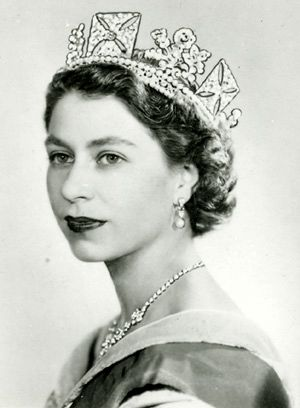
\includegraphics[width = 250px]{./picture/eli.jpg}
\end{center}

\end{figure}




\newpage

\tableofcontents

\newpage

\section{Introduction}

\vspace{1cm}

\subsection{Problématique et but du projet}

\vspace{1cm}

Le but de ce projet en programmation par contrainte est d'implementer un mini solveur pour des domaines CPSs finis.
La conception de ce projet s'étends sur trois séances de TP et doit nous permettre de proposer un solveur pour la recherche complète et la recherche local et comparer les solutions pour chaque méthode du problème dit "des n reines".

Nous avons décidé d'utiliser python 3.5.1 comme support de programmation et
nous traiterons dans une premiere partie du \textbf{Complete Search} et dans la seconde du \textbf{Local Search}.
Enfin, nous discuterons des résultats et de la comparaison de ceux ci dans la conclusion.


\vspace{1cm}

\subsection{le problème des n reines et les contraintes}

Le problème des n reines correspond à la mise en place de n reines sur un échiquier. Chaque reine ne doit pas être en position d'en attaquer une autre.
Il faut ainsi donc placer les reines d'une façon définie et respectant les contraintes suivante :

\begin{itemize}
\item Il doit y avoir qu'une reine par ligne.
\item Il doit y avoir qu'une reine par collone.
\item Il ne doit pas y avoir plus d'une reine par diagonal;
\end{itemize}


\begin{figure}[h]

\begin{center}
\includegraphics[]{./picture/prob.png}
\end{center}

\end{figure}


\newpage
\subsection{Compositiion de notre groupe}

\vspace{1cm}

\begin{tabbing}


\=blaaaaaaaaaaaa\=bmaaaaaaaaaaaaaaaaaaaaaaaaa   \=baaaaaaa\kill \\
\>Thibault 	\>Béziers La fosse		\>M1ALMA\\
\>Dennis	\>Bordet			\>M1ALMA\\
\>Joachim	\>Clayton			\>M1ALMA\\
\>Alexis	\>Giraudet			\>M1ALMA\\
\>Benjamin 	\>Moreau			\>M1ALMA\\


\end{tabbing}

\vspace{1cm}
\section{Partie 1 : Complete Search}
\vspace{2cm}

\subsection {Définition}

Le Complete Search est une méthode qui vise à rechercher une solution au problème en parcourant un arbre de possibilité progressivement remplie.
Celui ci utilise un algorithms de backtracking.

\subsection{}



\vspace{1cm}
\section{Partie 2 : Local Search}
\vspace{2cm}

\subsection {Définition}

Le Local Search elle est une méthode qui 

\subsection {}


\vspace{1cm}
\section{Conclusion}
\vspace{2cm}


\end{document}
